\section{The CMS Experiment}
The large hadron collider (LHC) in Geneva, Switzerland, is build to accelerate protons to very high velocities. In two adjacent beamlines, proton bunches travel in opposite directions around the ring. Eventually, those bunches collide in dedicated crossing points, which are surrounded by detectors. One of those detectors is the CMS experiment (see fig. \ref{cms}). CMS stands for Compact Muon Solenoid, a general-purpose detector. In the centre of the detector is the interaction point, where the proton-proton collisions occur.

Around this interaction point the different kinds of detectors are build in layers around the beamline. Those track and identify the particles produced by the proton-proton collision. The name giving solenoid magnet produces a magnetic field of 3.8\,T to curve the paths of the particles inside the detector. Inside the magnet volume is the tracker to identify the momentum of the particle and the electromagnetic followed by the hadronic calorimeter to measure the energy of various particles.  To detect muons, which penetrate the iron of the calorimeters, muon chambers are installed outside of the CMS magnet. \cite{CMS}

To be able to identify the angle of a particle relative to the beam axis, the pseudorapidity  ${\eta \equiv - \ln \left[ \tan \left( \frac{\theta}{2} \right) \right]}$ is used. Here $\theta$ gives the angle between the particle \mbox{impuls $\vec{p}$} and the positive direction of the beam axis.Typically particles with a high pseudorapidity are not measured, as they escape the detector alongside the beam. 
\begin{figure}
\centering
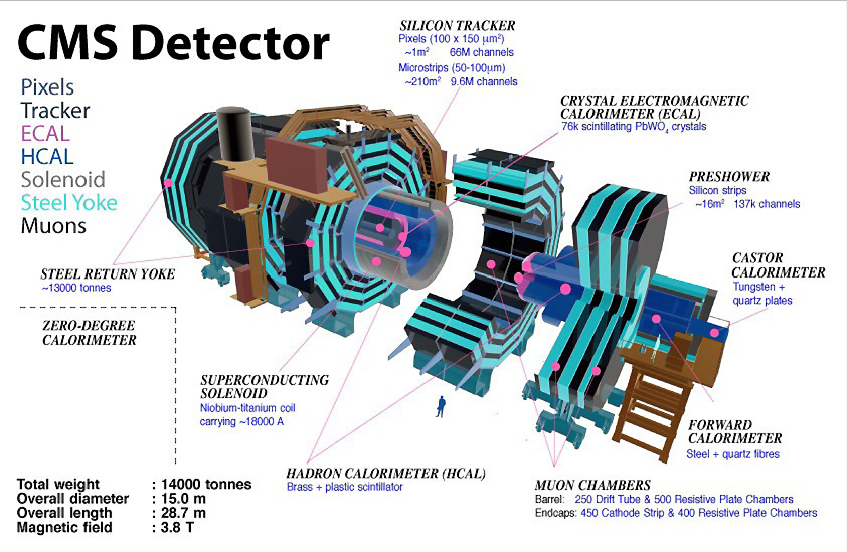
\includegraphics[scale=0.4]{cms_with_castor_drawing.jpg}
\caption{The CMS detector including its layers. The beam line is surrounded by the tracker and various calorimeters, as well as the superconducting solenoid and the muon chambers. CASTOR is located at the far right (source: \cite{CMSbild}).}
\label{cms}
\end{figure}

\section{The CASTOR Calorimeter}

The CASTOR calorimeter is part of the CMS detector. CASTOR stands for \enquote{Centauro And Strange Objects Research}. It is a very forward detector, covering the pseudorapidity range of -6.6 < $\eta$ < -5.2 . CASTOR is an electromagnetic and hadronic calorimeter which utilizes the Cherenkov effect to detect and classify particles. The calorimeter is divided into 16 sectors in azimuth and has 14 segments of readout units, or modules, along the longitudinal axis. The total number of channels is therefore 224. The 14 modules belonging to one sector are also called a tower.
The first two modules of every tower are electromagnetic readout units (EM modules) with a thickness of 7 mm each, which combine to 20.12 X$_0$. The remaining 12 modules form the hadronic calorimeter (HAD modules) with a thickness of 14 mm each, therefore with a length of 9.504 $\lambda_{\mathrm{I}}$. 
Its active material are quartz plates (2 mm thickness in the EM modules, 4 mm in the HAD modules) with tungsten absorbers inbetween (5 mm in EM, 10 mm in HAD modules). The entire detector has a length of 10.30 $\lambda_{\mathrm{I}}$, an inner radius of 3.7 cm and an outer radius of 14 cm. Outside of that the readout and infrastructure components are located, restricted to an outer radius of 30 cm given by the radiation shielding of CMS. Since CASTOR is therefore between the beam line and the radiation shield, it had to be built to withstand high radiation levels as well as high magnetic fields from the CMS magnet. 



If a particle produced by the initial collision at the interaction point reaches the calorimeter, it initiates a shower of secondary particles. These produce Cherenkov light, which can be detected by CASTOR. The quartz plates and tungsten absorbers have a 45$\degree$ inclination in respect to the beam axis to maximize the collection of Cherenkov light. The photons produced by the Cherenkov effect are then transmitted to photomultiplier tubes (PMTs) with the aid of air core lightguides. The PMTs transform the light into an electric signal. Each PMT corresponds to one of the 224 modules.
As the detector does not compensate the effect that electromagnetic particles produce more Cherenkov photons and therefore a higher energy response than hadronic particles, it is called a non-compensating calorimeter.



During high luminosity runs with p-p collisions CASTOR has to be removed from the beam line. As the detector is positioned very near the interaction point and due to its geometry it is impossible to evaluate pileup events. For that reason, to reduce the amount of radiation and to avoid back scattering of particles into CMS, CASTOR is removed during runs with high luminosity, where the number of collision per bunch crossing is higher than $\approx$ 1. For runs with low luminosity or Pb-Pb collisions it has to be installed. For this reason the detector can be split into two halves, each containing eight towers, to be removed from the beam line and then lifted up by a crane. \cite{castor}

\begin{figure}
\centering
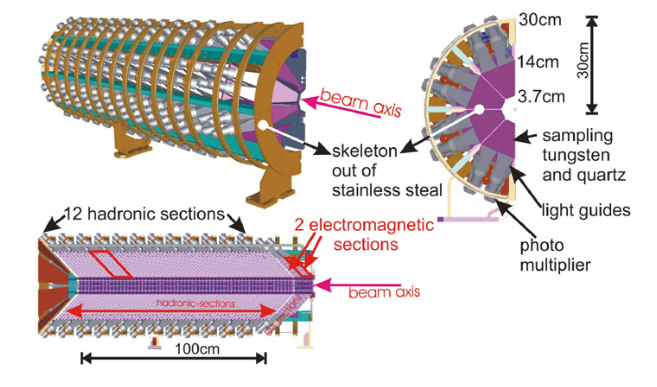
\includegraphics[scale=0.8]{castor.png}
\caption{The CASTOR	calorimeter. It is built in two parts around the beam line, with eight towers respectively, each tower containing two electromagnetic and twelve hadronic readout units. The readout units have a $45\degree$ inclination respective to the beam axis to maximize light collection (lower left) (source: \cite{castorbild}).}
\end{figure}
